\documentclass{report}

\usepackage[utf8]{inputenc}
\usepackage[T1]{fontenc}
\usepackage[francais]{babel}
\usepackage[top=2cm, bottom=2cm, left=3cm, right=3cm]{geometry}
\usepackage{color}
\usepackage{listings}
\usepackage{graphicx}


% Custom syntax highlighting
\definecolor{dkgreen}{rgb}{0,0.6,0}
\definecolor{gray}{rgb}{0.5,0.5,0.5}
\definecolor{mauve}{rgb}{0.58,0,0.82}

\lstset{language=C++,
    aboveskip=3mm,
    belowskip=3mm,
    showstringspaces=false,
    columns=flexible,
    basicstyle={\small\ttfamily},
    numbers=none,
    numberstyle=\tiny\color{gray},
    keywordstyle=\color{blue},
    commentstyle=\color{dkgreen},
    stringstyle=\color{mauve},
    breaklines=true,
    breakatwhitespace=true,
    tabsize=4
}
% end


\title{Rapport de projet NF05}
\author{Axel \bsc{Mousset} Aurélien \bsc{Labate}}

\begin{document}
    \maketitle

    \chapter{Choix technologiques}
    \chapter{Algorithmes utilisés}
        \section{Design pattern: Lexer/Parser}
            \begin{figure}[h]
                \begin{center}
                    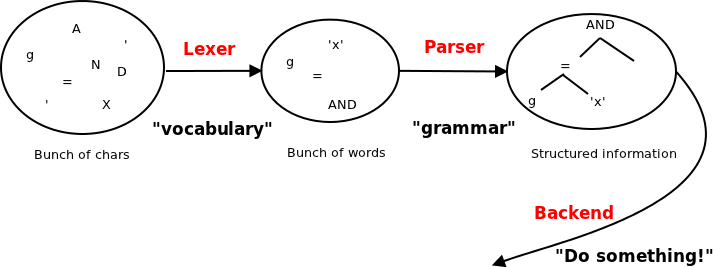
\includegraphics[scale=0.6]{./assets/lexer_parser.png}
                \end{center}

                \caption{Représentation du Lexer/Parser}
                \label{Représentation du Lexer/Parser}
            \end{figure}

            Lorem ipsum dolor sit amet, consectetur adipiscing elit. Nunc risus lectus, tincidunt eget odio sit amet, luctus scelerisque magna. Integer in arcu massa. Proin mattis dolor rhoncus orci suscipit molestie. Ut hendrerit ut elit in eleifend. Morbi suscipit diam purus, ut pulvinar velit auctor sed. Donec interdum pellentesque arcu vel dapibus. Donec et luctus sem. Mauris tincidunt nisi vel diam iaculis blandit. Vivamus facilisis mi in metus finibus, quis gravida nunc pretium.

            Sed nec congue tellus. Donec quis odio eget arcu pretium auctor. Donec sapien lacus, lacinia ullamcorper eleifend at, rutrum facilisis dui. Quisque posuere vel lectus vel tempor. In suscipit euismod aliquet. Quisque suscipit magna quam, a ultricies quam tristique ut. Donec tincidunt lectus faucibus quam tempus, vel aliquet lectus consectetur.

            Aliquam in lorem enim. Morbi et sollicitudin nibh, ut facilisis nibh. Nullam ornare nec risus dapibus vehicula. Nam porttitor sem et enim viverra, eget mattis ipsum tincidunt. Etiam vel vestibulum odio. Maecenas quis mi rutrum, convallis lectus ut, dapibus ipsum. Nam porta rutrum tincidunt. Maecenas suscipit tortor tortor, sit amet interdum felis consectetur et. Aliquam pellentesque sapien lacus, a hendrerit libero consequat sed. Nunc vel maximus massa. Pellentesque pulvinar at leo sit amet laoreet. Suspendisse sed metus est. Sed iaculis feugiat leo eu pharetra.

            Fusce consectetur elementum dui ac blandit. Praesent quis volutpat urna. Nulla quis nibh quis tellus dignissim sodales nec quis quam. Cras fermentum nunc vel suscipit mattis. Nam tincidunt pharetra massa sed ultricies. Nam tempor nibh quis leo porttitor, sit amet aliquet nisi molestie. In efficitur euismod nunc nec tempus. Pellentesque arcu purus, pharetra ut porttitor a, faucibus et nunc.

            Cras eu sapien tincidunt, venenatis nulla vitae, interdum turpis. Ut vitae justo sapien. Duis sed gravida orci. Quisque commodo accumsan accumsan. Nullam eu semper quam, vestibulum maximus diam. Cum sociis natoque penatibus et magnis dis parturient montes, nascetur ridiculus mus. Integer id efficitur erat. Nunc a libero fermentum tortor convallis sagittis a viverra leo. Etiam et turpis justo. Vivamus arcu urna, tristique in ipsum ornare, ornare tincidunt quam. Mauris pharetra euismod mollis

    \appendix
        \chapter{Code}
            % \lstinputlisting[language=C++]{../sources/mainwindow.cpp}
\lstinputlisting[language=C++]{../sources/detailedlist.cpp}
\lstinputlisting[language=C++]{../sources/mainwindow.hpp}
\lstinputlisting[language=C++]{../sources/about.cpp}
\lstinputlisting[language=C++]{../sources/detailedlist.hpp}
\lstinputlisting[language=C++]{../sources/about.h}
\lstinputlisting[language=C++]{../sources/main.cpp}
\lstinputlisting[language=C++]{../sources/lib/token.h}
\lstinputlisting[language=C++]{../sources/lib/calculables/matrix.cpp}
\lstinputlisting[language=C++]{../sources/lib/calculables/scalar.h}
\lstinputlisting[language=C++]{../sources/lib/calculables/matrix.h}
\lstinputlisting[language=C++]{../sources/lib/calculables/scalar.cpp}
\lstinputlisting[language=C++]{../sources/lib/assignationNode.cpp}
\lstinputlisting[language=C++]{../sources/lib/varNode.cpp}
\lstinputlisting[language=C++]{../sources/lib/calculable.h}
\lstinputlisting[language=C++]{../sources/lib/lexer.cpp}
\lstinputlisting[language=C++]{../sources/lib/node.h}
\lstinputlisting[language=C++]{../sources/lib/calculable.cpp}
\lstinputlisting[language=C++]{../sources/lib/parser.cpp}
\lstinputlisting[language=C++]{../sources/lib/token.cpp}
\lstinputlisting[language=C++]{../sources/lib/operator.h}
\lstinputlisting[language=C++]{../sources/lib/parser.h}
\lstinputlisting[language=C++]{../sources/lib/expressionNode.cpp}
\lstinputlisting[language=C++]{../sources/lib/operator.cpp}
\lstinputlisting[language=C++]{../sources/lib/assignationNode.h}
\lstinputlisting[language=C++]{../sources/lib/expressionNode.h}
\lstinputlisting[language=C++]{../sources/lib/varNode.h}
\lstinputlisting[language=C++]{../sources/lib/lexer.h}
\lstinputlisting[language=C++]{../sources/lib/node.cpp}
 to include all source codes
\end{document}